
\documentclass[aspectratio=169]{beamer}

%\usepackage[table]{xcolor}
\mode<presentation> {
\setbeamercovered{transparent}
  \usetheme{Boadilla}

%  \usetheme{Pittsburgh}
%\usefonttheme[2]{sans}
\renewcommand{\familydefault}{cmss}
%\usepackage{lmodern}
%\usepackage[T1]{fontenc}
%\usepackage{palatino}
%\usepackage{cmbright}
\usepackage{bm}
\usepackage{listings}
\usepackage{booktabs,adjustbox}
\useinnertheme{rectangles}
}
\usepackage{amsmath}
\setbeamercolor{normal text}{fg=black}
\setbeamercolor{structure}{fg= blue}
\definecolor{trial}{cmyk}{1,0,0, 0}
\definecolor{trial2}{cmyk}{0.00,0,1, 0}
\definecolor{darkgreen}{rgb}{0,.4, 0.1}
\definecolor{darkpurple}{rgb}{0.4, 0, 0.6}
\usepackage{array}
\beamertemplatesolidbackgroundcolor{white}  \setbeamercolor{alerted
text}{fg=darkpurple}
\usepackage{tcolorbox}
\setbeamertemplate{caption}[numbered]\newcounter{mylastframe}

\font\domino=domino
\def\die#1{{\domino#1}}
\usepackage{tikz}
\usetikzlibrary{arrows}
\usepackage{colortbl}

\renewcommand{\familydefault}{cmss}
%\usepackage[all]{xy}

\usepackage{tikz}
\usepackage{lipsum}

 \newenvironment{changemargin}[3]{%
 \begin{list}{}{%
 \setlength{\topsep}{0pt}%
 \setlength{\leftmargin}{#1}%
 \setlength{\rightmargin}{#2}%
 \setlength{\topmargin}{#3}%
 \setlength{\listparindent}{\parindent}%
 \setlength{\itemindent}{\parindent}%
 \setlength{\parsep}{\parskip}%
 }%
\item[]}{\end{list}}
\usetikzlibrary{arrows,shapes.geometric,shapes.misc,positioning}

\lstset{%
  language=R,
  basicstyle=\ttfamily\small,
  keywordstyle=\color{blue},
  commentstyle=\color{darkgreen},
  stringstyle=\color{darkpurple},
  showstringspaces=false,
  breaklines=true,
  frame=single,
  backgroundcolor=\color{gray!10}
}

\usecolortheme{lily}

\newtheorem{com}{Comment}
\newtheorem{lem} {Lemma}
\newtheorem{prop}{Proposition}
\newtheorem{condition}{Condition}
\newtheorem{thm}{Theorem}
\newtheorem{defn}{Definition}
\newtheorem{cor}{Corollary}
\newtheorem{obs}{Observation}
 \numberwithin{equation}{section}
 
\makeatletter
\def\beamerorig@set@color{%
  \pdfliteral{\current@color}%
  \aftergroup\reset@color
}
\def\beamerorig@reset@color{\pdfliteral{\current@color}}
\makeatother
\setbeamertemplate{navigation symbols}{}

\useoutertheme{miniframes}
\title[PLSC 30700]{Linear Models Lecture 18: Random Effects}

\author{Robert Gulotty}
\institute[Chicago]{University of Chicago}
\vspace{0.3in}


\begin{document}


\begin{frame}
\maketitle
\end{frame}



\begin{frame}{panelView}
\includegraphics[width=6 in]{../../RVersions/Panel/Rplot08.pdf}
\end{frame}
%
%\begin{frame}{Pre-test analysis}
%\begin{itemize}
%\item Suppose you run a model and find a variable is not significant or has the "wrong sign", so you drop it or add a control and re-estimate the model on the same data.
%\item Suppose you run a model and see an insignificant F test, discover you should have logged the DV, so you do and rerun the model on the same data.
%\item Suppose you find errors are serially dependent with a Durbin Watson statistic, so you run a Cochrane Orcutt estimator.
%\pause
%\item Conditioning on past test results will drive down p-values and produce estimates that appear to have high explanatory power even if X is totally unrelated to Y.
%\end{itemize}
%\end{frame}
%
%\begin{frame}{Better Practices}
%\begin{itemize}
%\item Begin with a theory informed target of inference.
%\item Form a theory informed statistical model.
%\item "Out of sample tests": adjust non-theoretical aspects of model on subset of data.
%\item Transparency/Pre-registration: Specify tests and decision rules in advance.
%\end{itemize}
%\end{frame}
%

\section{Random effects}
\begin{frame}{Motivation for Random Effects/ Partial Pooling}

\begin{itemize}
\item Given a model $y_{it}=\beta_0+\beta_1x_{it}+\alpha_i+e_{it}$, assume that 
\begin{enumerate}
\item Strict exogeneity holds: $E[e_i|\alpha_i,\bm{x}_{i1},\bm{x}_{i2},\ldots \bm{x}_{iT}]=0\ \quad \forall i$ 
\item The unobserved features are uncorrelated with $\bm{X}.$ $E[\alpha_i|\bm{x}_{i1},\bm{x}_{i2},\ldots \bm{x}_{iT}]=\alpha_0\ \quad \forall i$.
\end{enumerate}
\item Pooled OLS is consistent under 1), but we can do more (derive a more efficient estimator) with assumption 2).
\item Under 2) we can use the group structure to 
\begin{itemize}
\item rebalance the between and within estimator, dragging estimates toward group means,
\item use information about variables that do not vary within unit,
\item make predictions about unobserved groups.
\end{itemize}
\item This comes at the cost of introducing bias if 2) is false, ie, we failed to control for some time-invariant characteristic.
\end{itemize}
\end{frame}


\begin{frame}{Aitken (1935) Generalized Least Squares}
\begin{itemize}
\item We will use group structure to model dependence between observations.
$$\text{var}[\bm{e}|\bm{X}]=\Sigma\sigma^2$$
\item If we know $\Sigma$, we can do no better than to premultiply our linear model with  $\Sigma^{-1/2}$,
\begin{align*}
\bm{Y}&=\bm{X\beta}+\bm{e}\\
\Sigma^{-1/2}\bm{Y}&=\Sigma^{-1/2}\bm{X\beta}+\Sigma^{-1/2}\bm{e}\\
\bm{\tilde{Y}}&=\bm{\tilde{X}\beta}+\bm{\tilde{e}}\\\pause
\bm{\tilde{\beta}}_{GLS}&=(\bm{\tilde{X}'\tilde{X}})^{-1}\bm{\tilde{X}'\tilde{Y}}\\
&=((\Sigma^{-1/2}\bm{X})'(\Sigma^{-1/2}\bm{X}))^{-1}(\Sigma^{-1/2}\bm{X})'(\Sigma^{-1/2}\bm{Y})\\
&=(\bm{X}'\Sigma^{-1}\bm{X})^{-1}\bm{X}'\Sigma^{-1}\bm{Y}
\end{align*}
Here we have $E[\bm{\tilde{\beta}}_{GLS}]=\bm{\beta}$ and 
$var(\bm{\tilde{\beta}}_{GLS})=\sigma^2(\bm{X}'\Sigma^{-1}\bm{X})^{-1}$
\end{itemize}
\end{frame}

\begin{frame}{Random Effects Assumption}
\begin{columns}
\begin{column}{0.5\textwidth}
\begin{itemize}
\item The random effects assumption is that $Cov[\alpha_i, \bm{x}_{it}]=0$.
\item That is, we can consistently estimate our results in the cross-section.
\item Here is a picture where that is violated.
\end{itemize}
\end{column}
\begin{column}{0.5\textwidth}
\includegraphics[width=2.5 in]{ViolationofRandom.pdf}
\end{column}
\end{columns}
\end{frame}

\begin{frame}{Random Effects Assumption}
\begin{itemize}
\item Define a composite error term $\nu_{it}=\alpha_i+e_{it}$.
$$y_{it}=\bm{\beta}'\bm{x}_{it}+\alpha_i+e_{it}=\bm{\beta}'\bm{x}_{it}+\nu_{it}$$\pause
\begin{align*}
Var(\nu_{it})&=E[(\alpha_i+e_{it})^2]=E[\alpha_i^2+2\alpha_ie_{it}+e_{it}^2]=\sigma_\alpha^2+\sigma_e^2\\ \pause
Cov(\nu_{it}\nu_{is})&=E[\nu_{it}\nu_{is}]=E(\alpha_i+e_{it})(\alpha_i+e_{is})\\
&=E(\alpha_i^2+\alpha_ie_{it}+\alpha_ie_{is}+e_{it}e_{is})=E(\alpha_i^2)=\sigma_\alpha^2 \ \quad \forall t\neq s
\end{align*}
\item Recall correlation is $\rho=cov(x,y)/\sqrt{var(x)var(y)}$\pause
$$\rho_{\nu_{it}\nu_{is}}=\frac{\sigma_\alpha^2}{\sqrt{(\sigma_\alpha^2+\sigma_e^2)(\sigma_\alpha^2+\sigma_e^2)}}=\frac{\sigma_\alpha^2}{(\sigma_\alpha^2+\sigma_e^2)}$$
\end{itemize}
\end{frame}


\begin{frame}{Building Blocks}
Suppose that $\bm{\nu}_i=\begin{pmatrix}\nu_{i1}\\\nu_{i2}\\ \vdots\\ \nu_{iT}\end{pmatrix}$ for a generic individual $i$.

\begin{align*}
\underset{(T\times T)}{E(\bm{\nu}_i\bm{\nu}_i')}&=\begin{pmatrix} \sigma_\alpha^2+\sigma_e^2&\sigma^2_\alpha& \ldots &\sigma^2_\alpha\\
 \sigma_\alpha^2& \sigma_\alpha^2+\sigma_e^2& \ldots& \sigma^2_\alpha\\
 \ldots\\
 \sigma^2_\alpha& \sigma^2_\alpha& \ldots& \sigma_\alpha^2+\sigma_e^2\end{pmatrix}\\
 &= \sigma_e^2 \bm{I}+\sigma_\alpha^2\bm{i}\bm{i}'\\
 &=\bm{\Omega}
 \end{align*}
\end{frame}

\begin{frame}{Stacking people}
 Stacking individuals $\bm{\nu}=\begin{pmatrix}\bm{\nu}_{1}\\\bm{\nu}_{2}\\ \vdots\\\bm{\nu}_{t}\end{pmatrix}$ :
 $$\underset{(NT\times NT)}{E[ \bm{\nu}\bm{\nu}']}=\begin{pmatrix}\bm{\Omega}&\bm{0}&\bm{0}&\ldots\\ \bm{0}&\bm{\Omega}&\bm{0}\\ \bm{0}& \bm{0}&\bm{\Omega}&\\ \ldots \end{pmatrix}=\bm{\Omega}\otimes\bm{I}$$
\end{frame}





\begin{frame}{Theoretical GLS: Random Effects Estimation}
Using the fact that $var(\bm{\nu})=\bm{\Omega}\otimes\bm{I}$, we can apply GLS
$$\hat{\beta}_{RE}=(\bm{X}'(\bm{\Omega}\otimes\bm{I})^{-1}\bm{X})^{-1}\bm{X}'(\bm{\Omega}\otimes\bm{I})^{-1}\bm{y}$$
But we need estimates of  $\sigma^2_\nu$, $\sigma_e^2$ and $\sigma_\alpha^2$
$$\sigma^2_\nu=\sigma_e^2+\sigma_\alpha^2$$
\end{frame}

\begin{frame}{FGLS for Random Effects}
\begin{itemize}
\item Run OLS on pooled data and estimate residuals: $\hat{\nu}$
$$\widehat{\sigma^2_\nu}=\frac{\sum_{i=1}^N\sum_{t=1}^T \hat{\nu}_{it}^2}{NT-k}$$
\item We still need estimate of either $\sigma^2_\alpha$ or $\sigma^2_e$.
\item Wooldridge approach: take an average of observed covariances:
$$E\left( \frac{\sum_{s=1}^{T-1}\sum_{t=s+1}^{T}\hat{\nu}_{is}\hat{\nu}_{it}}{N\frac{(T-1)T}{2}-k}\right)=\sigma_\alpha^2$$
$$\widehat{\sigma}^2_\nu-\widehat{\sigma}_\alpha^2=\widehat{\sigma}_e^2$$
\end{itemize}
\end{frame}

\begin{frame}{Partial Pooling}
\begin{itemize}
\item Random effects models are partial pooling:
$$\bm{b}_{RE}=\bm{\lambda}\bm{b}_W+(\bm{I}-\bm{\lambda})\bm{b}_B$$
$$\bm{\lambda}=(\bm{S}^W_{xx}+(1-\theta^2)\bm{S}_{xx}^B)^{-1}\bm{S}_{xx}^W$$
\item Here $\theta$ is between 0 and 1.  Under random effects:
$$\theta=1-\sqrt{\frac{\sigma^2_e}{\sigma^2_e+T\sigma^2_\alpha}}$$
$$\theta=1-\sqrt{\frac{1}{1+T(\sigma^2_\alpha/\sigma^2_e)}}$$
\end{itemize}
\end{frame}



\begin{frame}{Comparing Fixed vs Random Effects}
\begin{itemize}
\item Random effects
\begin{itemize}
\item Is efficient.
\item Allows analysis of time-constant variables.
\item Allows extrapolation to unobserved groups.
\item Assumes $\bm{X}$ is independent of $\alpha$
\item plm(y $\sim$ x, data = dta, index = c("id", "year"), model = "random")
\end{itemize}
\item Fixed effects
\begin{itemize}
\item Washes out time-constant variables.
\item Uses many $n$ degrees of freedom.
\item Allows any sort of relationship between $\bm{X}$ and $\alpha$
\item plm(y $\sim$ x, data = dta, index = c("id", "year"), model = "within")
\end{itemize}
\end{itemize}
\end{frame}



\section{Testing Random effects}
\begin{frame}{Hausman (1978) Specification Test}
\begin{itemize}
  \item \textbf{Idea:} compare FE and RE estimates of $\bm{\beta}$.
    \begin{itemize}
      \item Under $H_0$ (RE valid): both consistent, RE more efficient $\;\Rightarrow\;$ difference is small.
      \item Under $H_1$ (RE invalid): RE inconsistent, FE still consistent $\;\Rightarrow\;$ systematic difference.
    \end{itemize}\pause
  \item \textbf{Test statistic}
    \[
      H \;=\;
      \bigl(\hat{\bm{\beta}}_{FE}-\hat{\bm{\beta}}_{RE}\bigr)'
      \bigl[\widehat{\text{Var}}(\hat{\bm{\beta}}_{FE})
            -\widehat{\text{Var}}(\hat{\bm{\beta}}_{RE})\bigr]^{-1}
      \bigl(\hat{\bm{\beta}}_{FE}-\hat{\bm{\beta}}_{RE}\bigr)
      \;\;\xrightarrow{d}\;\;\chi^{2}_{K}
    \]
    where $K=\dim(\bm{\beta})$.  Reject $H_0$ when $H$ is large.\pause
  \item \textbf{GMM connection:} This is a special case of the GMM endogeneity test (Hansen, Thm 13.16, Lecture 16). The GMM version replaces the classical variance difference with a robust sandwich estimator, making it valid under heteroskedasticity.
\end{itemize}
\end{frame}

\begin{frame}[fragile]{Hausman Test in Practice}
\lstset{language=R,basicstyle=\ttfamily\scriptsize,
  keywordstyle=\color{blue},commentstyle=\color{gray},
  columns=flexible,keepspaces=true,showstringspaces=false}
\begin{lstlisting}
fe_mod <- plm(log(gsp) ~ log(pcap) + log(hwy) + log(util),
              data = pdata, model = "within")
re_mod <- plm(log(gsp) ~ log(pcap) + log(hwy) + log(util),
              data = pdata, model = "random")

phtest(fe_mod, re_mod)   # classical Hausman chi-squared
\end{lstlisting}
\begin{itemize}
  \item \textbf{Caveat:} This is a \emph{specification test}, not a model-selection tool.
  \item Using it to choose FE vs.\ RE makes your estimator a
        \emph{pretest estimator} $\;\Rightarrow\;$ biases subsequent inference.\pause
  \item Better alternatives when unsure:
    \begin{itemize}
      \item Use FE (conservative).
      \item Use \textbf{Correlated Random Effects} (Mundlak), which nests both
            and supplies a robust version of the same test.
    \end{itemize}
\end{itemize}
\end{frame}

\section{Correlated Random Effects}
%---------------------------------------------------------------
% Frame 1 —  Why time-invariant covariates are a headache
\begin{frame}{Time-Invariant Regressors: the Identification Problem}
\begin{itemize}
  \item[] \textbf{Panel baseline}  
    \[
      y_{it} \;=\; \bm{x}_{it}'\bm{\beta} \;+\; \bm{z}_{i}'\bm{\gamma}
      \;+\; \alpha_i \;+\; e_{it},
      \qquad i=1,\dots,N,\; t=1,\dots,T
    \]
    \begin{itemize}
      \item $\bm{x}_{it}$ : time-varying covariates  
      \item $\bm{z}_{i}$  : \textit{time-invariant} covariates  
      \item $\alpha_i$    : unit fixed effect, unobserved and potentially \emph{correlated} with $\bm{x}_{it},\bm{z}_{i}$
    \end{itemize}\pause
  \item The \alert{within transformation} eliminates $\alpha_i$ but also wipes out
        $\bm{z}_{i}$ (no variation over~$t$) $\;\Rightarrow\;$ standard FE cannot identify coefficients on $\bm{z}_{i}$.
  \item E.g. we want to know the coefficient on colonial legacy, ethnic fractionalization, or distance to Russia.
\end{itemize}
\end{frame}

%---------------------------------------------------------------
% Frame 2 —  Two model-based solutions (Bruce Hansen style summary)
\begin{frame}{Model-Based Remedies for $\bm{z}_{i}$}
\begin{itemize}
  \item \textbf{Correlated Random Effects (Mundlak, 1978)}
    \begin{itemize}
      \item Model the dependence of $\alpha_i$ on the \emph{time-varying} regressors:
            $\displaystyle \alpha_i \;=\;
              \delta_0 \;+\; \bar{\bm{x}}_{i}'\bm{\delta} \;+\; \zeta_i$,
            \quad $\bar{\bm{x}}_{i}\equiv T^{-1}\!\sum_{t}\bm{x}_{it}$.
      \item Conditional on $\bar{\bm{x}}_{i}$, treat $\zeta_i$ as \emph{random}:
            $\mathbb{E}[\zeta_i\mid\bm{x}_{it},\bm{z}_{i}]=0$.
      \item Estimation via GLS delivers FE-consistent
            $\hat{\bm{\beta}}$ and identifies $\bm{\gamma}$ on $\bm{z}_i$.
    \end{itemize}\pause
  \item \textbf{Hausman--Taylor (1981)}
    \begin{itemize}
      \item Partition regressors
        $\bm{x}_{it}=(\bm{x}_{1it},\bm{x}_{2it}),\;
         \bm{z}_{i}=(\bm{z}_{1i},\bm{z}_{2i})$
        such that
        \(
          \bm{x}_{1it},\bm{z}_{1i}
        \) are exogenous,
        \(
          \bm{x}_{2it},\bm{z}_{2i}
        \) possibly endogenous.
      \item Use \(\bm{x}_{1it}\) (within variation) and \(\bm{z}_{1i}\)
            (between variation) as instruments for \(\bm{x}_{2it},\bm{z}_{2i}\).
      \item Two-step IV--GLS attains efficiency under random-effects covariance.
    \end{itemize}
\end{itemize}
\end{frame}

%---------------------------------------------------------------
% Frame 3 —  Correlated Random Effects à la Mundlak
\begin{frame}{Correlated Random Effects (Mundlak)}
\begin{itemize}
  \item \textbf{Structural restriction}
    \[
      \alpha_i \;=\; \delta_0 \;+\; \bar{\bm{x}}_{i}'\bm{\delta} \;+\; \zeta_i,
      \qquad \mathbb{E}[\zeta_i\mid\bm{x}_{it},\bm{z}_{i}]=0
    \]
    where $\bar{\bm{x}}_{i}= T^{-1}\!\sum_{t}\bm{x}_{it}$.
    All correlation between $\alpha_i$ and the time-varying covariates is
    absorbed by $\bar{\bm{x}}_{i}'\bm{\delta}$.\pause
  \item Substituting into the panel model:
    \[
      y_{it}
      \;=\;
      \bm{x}_{it}'\bm{\beta}
      \;+\;
      \bm{z}_{i}'\bm{\gamma}
      \;+\;
      \delta_0 + \bar{\bm{x}}_{i}'\bm{\delta}
      \;+\;
      \underbrace{\zeta_i + e_{it}}_{\text{composite error}}
    \]\pause
  \item Apply GLS (random-effects weighting) to the augmented model.
    \begin{itemize}
      \item $\hat{\bm{\beta}}$ identical to FE (we will see why via FWL).
      \item $\hat{\bm{\gamma}}$ on $\bm{z}_i$ is now identified.
      \item Testable implication:
        $H_0\!:\;\bm{\delta}=\bm{0}$ reduces CRE to conventional RE.
    \end{itemize}
\end{itemize}
\end{frame}

%---------------------------------------------------------------
% Frame 3b — FWL intuition for CRE = FE
\begin{frame}{Why $\hat{\bm{\beta}}_{CRE} = \hat{\bm{\beta}}_{FE}$: FWL Intuition}
\begin{itemize}
  \item The CRE regression includes $\bm{x}_{it}$, $\bar{\bm{x}}_i$,
        $\bm{z}_i$, and a constant.
  \item By the \textbf{Frisch--Waugh--Lovell theorem}, the coefficient on
        $\bm{x}_{it}$ is obtained by first \emph{partialing out}
        $\bar{\bm{x}}_i$ (and $\bm{z}_i$, constant) from both $y_{it}$
        and $\bm{x}_{it}$.\pause
  \item Partialing $\bar{\bm{x}}_i$ from $\bm{x}_{it}$:
    \[
      \bm{x}_{it} - \bar{\bm{x}}_i
      \;=\; \text{within-demeaned data}
    \]
  \item So $\hat{\bm{\beta}}_{CRE}$ uses \emph{only within-unit variation}
        --- exactly the same variation that FE uses.\pause
  \item \textbf{Bonus:} CRE also identifies $\bm{\gamma}$ (the coefficient on
        $\bm{z}_i$) because $\zeta_i$ is uncorrelated with all regressors
        by assumption.
\end{itemize}
\end{frame}

%---------------------------------------------------------------
% Frame 3c — Mundlak test = Hausman test
\begin{frame}{The Mundlak Test $=$ Hausman Test}
\begin{itemize}
  \item From the CRE regression, test
    \[
      H_0\!:\; \bm{\delta} = \bm{0}
      \qquad\text{(unit means have no additional explanatory power)}
    \]
  \item Under $H_0$: $\alpha_i$ uncorrelated with $\bm{x}_{it}$
        $\;\Rightarrow\;$ standard RE is valid.
  \item Under $H_1$: RE is inconsistent, but CRE (= FE for $\bm{\beta}$)
        remains consistent.\pause
  \item A standard $F$-test (or Wald test) on $\bm{\delta}=\bm{0}$ is
        \textbf{numerically equivalent} to the classical Hausman $\chi^2$.
  \item \textbf{Advantage:} the CRE version
    \begin{itemize}
      \item is easy to compute (just an $F$-test on extra regressors),
      \item works with \emph{robust / clustered} standard errors
            (the classical Hausman test does not).
    \end{itemize}
\end{itemize}
\end{frame}

\begin{frame}[fragile]{R implementation: Mundlak CRE}
\lstset{ %
  language        = R,
  basicstyle      = \ttfamily\scriptsize,
  keywordstyle    = \color{blue},
  commentstyle    = \color{gray},
  columns         = flexible,
  keepspaces      = true,
  showstringspaces=false
}
\begin{lstlisting}
library(plm)                     # panel-data toolkit
data("Produc", package = "Ecdat")# US state production data

dffrost<-data.frame( state = str_replace(toupper(rownames(state.x77)),"\\s","_"),
frost = state.x77[,"Frost"])%>%mutate(state=ifelse(state=="TENNESSEE", "TENNESSE",state))

Producweather<-Produc%>%left_join(dffrost)
pdata <- pdata.frame(Producweather, index = c("state", "year"))

pdata$pcap_bar <- Between(log(pdata$pcap))   # == ave(pcap, state)
pdata$hwy_bar <- Between(log(pdata$hwy))
pdata$util_bar<- Between(log(pdata$util))

cre_mod <- plm(log(gsp) ~ log(pcap)+log(hwy)+log(util)+pcap_bar+hwy_bar+util_bar+frost,
               data   = pdata,
               model  = "random")     # GLS w/ error-components

fe_mod <- plm(log(gsp) ~ log(pcap)+ log(hwy)+log(util),
               data   = pdata,
               model  = "within")  
               
\end{lstlisting}
\end{frame}


% -----------------------------------------
\begin{frame}{Regression results}
\scriptsize           % or \footnotesize
\centering
\begin{adjustbox}{max totalsize={\textwidth}{0.8\textheight},center}
\begin{tabular}{@{}lcc@{}}
\toprule
                     & \textbf{Model 1} & \textbf{Model 2} \\
\midrule
Intercept            & 0.14            &                  \\
                     & (0.65)          &                  \\[2pt]

\textit{Time-varying covariates} \\[2pt]
log(pcap)            & 2.26$^{***}$    & 2.26$^{***}$     \\
                     & (0.15)          & (0.15)           \\
log(hwy)             & –0.81$^{***}$   & –0.81$^{***}$    \\
                     & (0.11)          & (0.11)           \\
log(util)            & –0.47$^{***}$   & –0.47$^{***}$    \\
                     & (0.08)          & (0.08)           \\[2pt]

\textit{Means} \\[2pt]
pcap\_bar            & –1.19           &                  \\
                     & (0.81)          &                  \\
hwy\_bar             & 0.87            &                  \\
                     & (0.45)          &                  \\
util\_bar            & 0.41            &                  \\
                     & (0.40)          &                  \\
\textit{Time invariant} \\[2pt]
frost                & –0.00           &                  \\
                     & (0.00)          &                  \\[2pt]

$\sigma_\text{idios}$ & 0.08            &                  \\
$\sigma_\text{id}$    & 0.18            &                  \\[4pt]

$R^{2}$              & 0.81            & 0.71             \\
Adj.\ $R^{2}$        & 0.81            & 0.69             \\
Observations         & 816             & 816              \\
\bottomrule
\multicolumn{3}{@{}l@{}}{\footnotesize
  $^{***}p<0.001$;\; $^{**}p<0.01$;\; $^{*}p<0.05$}
\end{tabular}
\end{adjustbox}
\end{frame}


%---------------------------------------------------------------
% Two-Way Mundlak
\begin{frame}{Two-Way Mundlak (Wooldridge, 2021)}
\begin{itemize}
  \item With unit \emph{and} time fixed effects:
    $y_{it} = \bm{x}_{it}'\bm{\beta} + \alpha_i + \lambda_t + e_{it}$
  \item \textbf{Two-way Mundlak:} include both \emph{unit means} $\bar{\bm{x}}_{i\cdot}$
        and \emph{time means} $\bar{\bm{x}}_{\cdot t}$ as additional regressors
        in a pooled or RE regression.\pause
  \item Delivers TWFE-equivalent $\hat{\bm{\beta}}$ while allowing
    \begin{itemize}
      \item time-invariant regressors ($\bm{z}_i$) and
      \item unit-invariant regressors ($\bm{w}_t$).
    \end{itemize}\pause
  \item \textbf{Key application:} staggered difference-in-differences with
        heterogeneous treatment effects.
    \begin{itemize}
      \item Standard TWFE can assign \emph{negative weights} to some
            treatment effects.
      \item Two-way Mundlak avoids this problem by explicitly modeling the
            dependence structure.
    \end{itemize}
\end{itemize}
\end{frame}

\begin{frame}{Robust Standard errors}
\begin{itemize}
\item Newey-West, like White with a specified lag, adjusts for autocorrelation and heteroskedasticity.  \texttt{vcovNW}
\item Beck-Katz, use large-T asymptotics to correct for cross-sectional dependence: good for if T/N is not too small. \texttt{vcovBK}
\item Driscoll-Kraay applies Newey-West to cross-sectional dependence: good if if T/N is small. \texttt{vcovSCC}
\end{itemize}
\end{frame}

\section{Dynamic Panel GMM}

\begin{frame}{The Dynamic Panel Problem}
\begin{itemize}
\item Many panel models include a lagged dependent variable:
$$Y_{it}=\rho Y_{it-1}+\bm{X}_{it}'\bm{\beta}+\alpha_i+e_{it}$$\pause
\item \textbf{Problem:} the within transformation creates correlation between the transformed lagged DV and the transformed error (Nickell, 1981):
$$\tilde{Y}_{it-1}=(Y_{it-1}-\bar{Y}_i) \quad\text{is correlated with}\quad \tilde{e}_{it}=(e_{it}-\bar{e}_i)$$
because $\bar{Y}_i$ contains $Y_{it}$ which depends on $e_{it}$, and $\bar{e}_i$ contains $e_{it-1}$ which affects $Y_{it-1}$.\pause
\item The bias is $O(1/T)$: severe when $T$ is small (typical in micro panels), vanishes as $T\to\infty$.
\item \textbf{FE is inconsistent} for fixed $T$ with a lagged dependent variable.
\end{itemize}
\end{frame}

\begin{frame}{Arellano-Bond: First Differencing + Instruments}
\begin{itemize}
\item \textbf{Step 1:} First-difference to eliminate $\alpha_i$:
$$\Delta Y_{it}=\rho\,\Delta Y_{it-1}+\Delta\bm{X}_{it}'\bm{\beta}+\Delta e_{it}$$\pause
\item \textbf{Step 2:} $\Delta Y_{it-1}$ is correlated with $\Delta e_{it}$ (since $Y_{it-1}$ appears in both).\\
Use \alert{lagged levels} as instruments: $Y_{is}$ for $s\leq t-2$.\pause
\item \textbf{Moment conditions:}
$$E[Y_{is}\cdot \Delta e_{it}]=0 \quad\text{for } s\leq t-2$$
\item At $t=3$: one instrument ($Y_{i1}$). At $t=4$: two ($Y_{i1},Y_{i2}$). At $t=T$: $T-2$ instruments.
\item Total moment conditions: $\frac{(T-1)(T-2)}{2}$ --- the system is \textbf{overidentified} $\Rightarrow$ GMM.
\end{itemize}
\end{frame}

\begin{frame}{Arellano-Bond as GMM}
\begin{itemize}
\item This is exactly the GMM framework from Lectures 15--16:\pause
\begin{enumerate}
\item \textbf{Step 1:} Estimate with a preliminary weight matrix (e.g., $\bm{W}=(\bm{Z}'\bm{H}\bm{Z})^{-1}$ where $\bm{H}$ is a first-difference covariance structure).
\item \textbf{Step 2:} Re-estimate using the optimal weight matrix from step 1 residuals (two-step GMM).
\end{enumerate}\pause
\item \textbf{$J$-test} (Hansen/Sargan): test the $\frac{(T-1)(T-2)}{2}-k$ overidentifying restrictions.
\begin{itemize}
\item $\text{df}=\text{moments}-\text{parameters}$
\item Rejection $\Rightarrow$ serial correlation in $e_{it}$ or invalid instruments.
\end{itemize}\pause
\item \textbf{Key diagnostic:} AR(2) test on differenced residuals.
\begin{itemize}
\item AR(1) in $\Delta e_{it}$ is expected by construction.
\item AR(2) in $\Delta e_{it}$ implies AR(1) in $e_{it}$ $\Rightarrow$ instruments invalid.
\end{itemize}
\end{itemize}
\end{frame}

\begin{frame}{Extensions and Practical Guidance}
\begin{itemize}
\item \textbf{System GMM} (Blundell-Bond, 1998): augments the differenced equations with \emph{level equations} instrumented by lagged differences.
\begin{itemize}
\item Additional moments: $E[\Delta Y_{is}\cdot(\alpha_i+e_{it})]=0$ for $s=t-1$.
\item Especially useful when the series is persistent ($\rho$ near 1), where Arellano-Bond instruments are weak.
\end{itemize}\pause
\item \textbf{Practical rules:}
\begin{itemize}
\item Designed for ``large $N$, small $T$'' panels.
\item Too many instruments $\Rightarrow$ overfitting. Collapse or limit lag depth.
\item Always report: (1) $J$-test $p$-value, (2) AR(2) test, (3) number of instruments vs.\ groups.
\end{itemize}\pause
\item \textbf{Software:} \texttt{plm::pgmm()} in R; \texttt{xtabond2} in Stata.
\begin{itemize}
\item \texttt{pgmm(y $\sim$ lag(y,1) + x | lag(y, 2:99), data=pdata, effect="twoways")}
\end{itemize}
\end{itemize}
\end{frame}

\begin{frame}{Application: Does Income Cause Democracy?}
\begin{itemize}
\item \textbf{Acemoglu, Johnson, Robinson \& Yared (2008):} Classic question --- does economic development promote democratization?
\item \textbf{Model:} $\text{Democracy}_{it}=\rho\,\text{Democracy}_{it-1}+\beta\,\text{Income}_{it-1}+\alpha_i+\lambda_t+e_{it}$\pause
\item \textbf{The problem with FE:} Democracy is highly persistent ($\rho\approx 0.7$).
\begin{itemize}
\item Within-transformation induces Nickell bias in $\hat{\rho}$ (biased toward zero).
\item This bias contaminates $\hat{\beta}$ as well.
\item With $T\approx 10$ (five-year panels), the bias is substantial.
\end{itemize}\pause
\item \textbf{Arellano-Bond solution:} First-difference to eliminate $\alpha_i$, then instrument $\Delta\text{Democracy}_{it-1}$ with lagged levels.
\item \textbf{Finding:} Once dynamic panel bias is corrected, the income effect on democracy becomes insignificant --- country fixed effects explain most of the cross-national correlation.
\end{itemize}
\end{frame}

\begin{frame}[fragile]{Arellano-Bond in R: Tax Progressivity Example}
\begin{lstlisting}[basicstyle=\ttfamily\scriptsize]
library(plm); library(haven)
dta <- read_dta("progressTax.dta")
pdta <- pdata.frame(subset(dta, year >= 1850),
                    index = c("ccode", "year"))

# Arellano-Bond: two-step GMM
ab_mod <- pgmm(
  topratep ~ lag(topratep, 1) + himobpopyear2p
    | lag(topratep, 2:99),
  data = pdta,
  effect = "twoways",    # unit + time effects
  model = "twosteps")    # two-step GMM
summary(ab_mod)

# Key diagnostics
summary(ab_mod)$sargan   # J-test (overid)
# Check AR(2) test: p > 0.05 validates
#   the moment conditions
\end{lstlisting}
\end{frame}

\begin{frame}[fragile]{Reading Arellano-Bond Output}
\begin{lstlisting}[basicstyle=\ttfamily\scriptsize]
summary(ab_mod)
# Coefficients:
#                  Estimate Std. Error z-value Pr(>|z|)
# lag(topratep,1)   0.xxx    0.xxx     x.xx    0.xxx
# himobpopyear2p    0.xxx    0.xxx     x.xx    0.xxx
#
# Sargan test: chisq(df) = xx, p-value = 0.xxx
#   (large p -> instruments valid)
# Autocorrelation test (2):  z = x.xx, p = 0.xxx
#   (large p -> no AR(2) in levels)
\end{lstlisting}
\smallskip
\textbf{Checklist for reporting:}
\begin{enumerate}\itemsep=1pt
\item $\hat{\rho}$: persistence of lagged DV (compare to FE estimate)
\item Sargan/Hansen $J$-test $p$-value $> 0.05$
\item AR(2) test $p$-value $> 0.05$
\item Number of instruments $<$ number of groups
\end{enumerate}
\end{frame}


\begin{frame}{Choosing a Panel Estimator}
\centering
\vspace{-6pt}
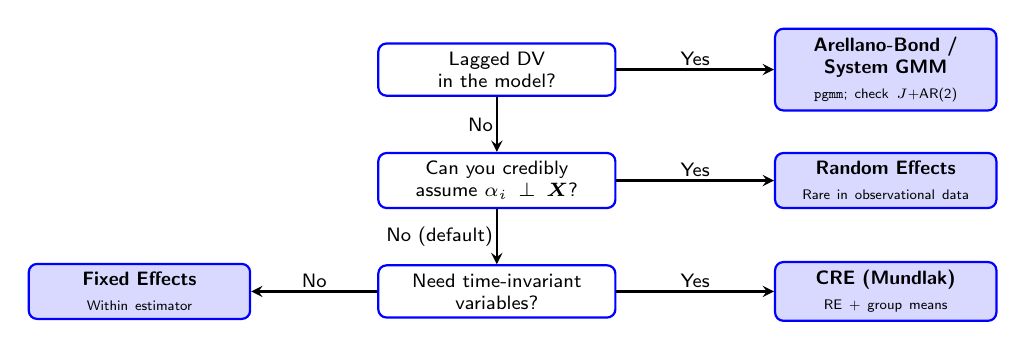
\begin{tikzpicture}[
  decision/.style={rectangle, rounded corners=3pt, draw=blue, thick,
    fill=white, text width=2.8cm, align=center, inner sep=3pt,
    font=\scriptsize},
  estimator/.style={rectangle, rounded corners=3pt, draw=blue, thick,
    fill=blue!15, text width=2.6cm, align=center, inner sep=3pt,
    font=\scriptsize},
  arr/.style={->, thick, >=stealth},
  lbl/.style={font=\scriptsize, fill=white, inner sep=1pt}
]

% Row 1: lagged DV?
\node[decision] (lagdv) {Lagged DV\\in the model?};

% Right branch: AB
\node[estimator, right=2.0cm of lagdv] (ab)
  {\alert{\textbf{Arellano-Bond /\\System GMM}}\\[1pt]
   \tiny\texttt{pgmm}; check $J$+AR(2)};

% Row 2: can you credibly assume independence?
\node[decision, below=0.7cm of lagdv] (corr)
  {Can you credibly\\assume $\alpha_i \perp \bm{X}$?};

% Left branch: default -- FE/CRE
\node[decision, below=0.7cm of corr] (tiv)
  {Need time-invariant\\variables?};

% Right branch: RE (the exception)
\node[estimator, right=2.0cm of corr] (re)
  {\alert{\textbf{Random Effects}}\\[1pt]
   \tiny Rare in observational data};

% Endpoints row 3
\node[estimator, left=1.6cm of tiv] (fe)
  {\alert{\textbf{Fixed Effects}}\\[1pt]
   \tiny Within estimator};
\node[estimator, right=2.0cm of tiv] (cre)
  {\alert{\textbf{CRE (Mundlak)}}\\[1pt]
   \tiny RE + group means};

% Arrows
\draw[arr] (lagdv) -- node[lbl, above] {Yes} (ab);
\draw[arr] (lagdv) -- node[lbl, left]  {No}  (corr);
\draw[arr] (corr)  -- node[lbl, above] {Yes} (re);
\draw[arr] (corr)  -- node[lbl, left]  {No (default)} (tiv);
\draw[arr] (tiv)   -- node[lbl, above] {No}  (fe);
\draw[arr] (tiv)   -- node[lbl, above] {Yes} (cre);

\end{tikzpicture}

\vspace{2pt}
{\scriptsize The choice of estimator should follow from your research design, not from a post-hoc test.}
\end{frame}


\begin{frame}{Why Not Let the Hausman Test Decide?}
\begin{itemize}
\item A common workflow: estimate FE and RE, run the Hausman test, pick the ``winner.''
\item This is \alert{pre-test estimation} --- your final estimator is selected by a preliminary test.
\pause
\item \textbf{Problem:} the sampling distribution of the reported estimate is a \emph{mixture} of the FE and RE distributions, weighted by the probability the test selects each one.
\item Standard errors and confidence intervals ignore the selection step $\Rightarrow$ \alert{undercoverage}.
\pause
\item \textbf{Better approach:} let your \textbf{research design} determine the estimator:
\begin{itemize}
\item Is selection into units plausibly correlated with covariates? (Almost always yes with observational country-, state-, or individual-panels.) $\Rightarrow$ FE or CRE.
\item Use the Hausman test as a \emph{diagnostic}, not a decision rule. Report it alongside your preferred specification.
\end{itemize}
\end{itemize}
\end{frame}


\begin{frame}{When Is Random Effects Reasonable?}
RE assumes $\alpha_i \perp \bm{X}_{it}$: unit heterogeneity is unrelated to covariates.\pause
\smallskip

\textbf{Plausible settings in political science:}
\begin{enumerate}\itemsep=1pt
\item \textbf{Randomized/quasi-random assignment across units} --- e.g., audit experiments in randomly sampled municipalities. Treatment is exogenous.
\item \textbf{Surveys with cluster sampling} --- individuals within randomly selected clusters. The cluster effect is a nuisance, not a confounder.
\item \textbf{Meta-analysis} --- studies are ``units''; heterogeneity is modeled as random for population-average inference.
\end{enumerate}\pause
\smallskip

\textbf{When to be skeptical (most observational panels):}
\begin{itemize}\itemsep=1pt
\item Countries self-select into trade agreements, wars, institutions.
\item States adopt policies endogenously.
\item Individuals sort into groups based on characteristics that also affect $Y$.
\end{itemize}
\smallskip
\alert{Default:} assume $\alpha_i$ is correlated with $\bm{X}$ and use FE or CRE unless you can argue otherwise.
\end{frame}


\begin{frame}{Discussion and Course Integration}
\begin{itemize}
\item Panel estimators fit into the \textbf{unified GMM framework} from Lectures 15--16:
\begin{itemize}
\item FE: within-group moment conditions (just-identified).
\item RE: adds between-group moments via GLS weighting (efficiency gain under $H_0$).
\item CRE (Mundlak): augmented RE that nests FE; Mundlak test $=$ Hausman test.
\item Arellano-Bond: lagged levels as instruments in first-differenced equations (overidentified $\Rightarrow$ $J$-test).
\end{itemize}\pause
\item You can use panel structure to improve efficiency (not discarding cross-unit variation) at the cost of bias if assumptions fail.
\item Many studies focus on slow-moving processes that cannot be estimated with pure fixed effects.
\item Dynamic panels require GMM-based approaches; the $J$-test provides a specification check that was not available with FE alone.
\end{itemize}
\end{frame}
%
%\section{Missing Data}
%\begin{frame}{Imputation?}
%\begin{itemize}
%\item R and Stata will, by default, drop any observation if any of the variables are missing.
%\item In Panel Data, this effects a single unit-year.
%\item Tradeoff between adding a control variable and reducing sample size.
%\item Need to assume missingness is random with respect to the statistical process.
%\item Typical imputation process:
%\begin{itemize}
%\item Use random forests to fill in values to produce 20x-100x datasets (missRanger)
%\item Run model on each dataset, record coefficients. (lapply)
%\item Average across datasets, accounting for variance across replications (mice::pool)
%\end{itemize}
%
%\end{itemize}
%\end{frame}
%


\end{document}